
The Inner Tracker (ITk) is an all-silicon detector that will completely replace the current Inner Detector.  While the current ID has been extremely successful during Runs 1 and 2 (and will certainly continue to be in Run 3), it does not have the capacity to withstand the radiation and pile-up conditions of the HL-LHC. The ITk is designed to operate for 10 years at an instantaneous luminosity of 7.5$\times10^{-34}$ cm$^{-2}$s$^{-1}$ with 25 ns between proton bunches. This will result in 1,000 fb$^{-1}$ and average pile-up up to $200$ \cite{ITktech}. The current solenoid magnet will remain in the detector providing a 2 T magnetic field. The ITk will consist of an innermost section with silicon pixels and an outermost section of silicon strips. The pixel detector will contain four barrel layers and six forward region disks, while the strip detector will contain five barrel layers and seven disks. The rapidity range matches the coverage of the Muon Spectrometer with $|\eta|<2.7$. This layout is shown in Figure~\ref{fig:ITklayout}. 
\begin{figure}[!h]
        \centering
    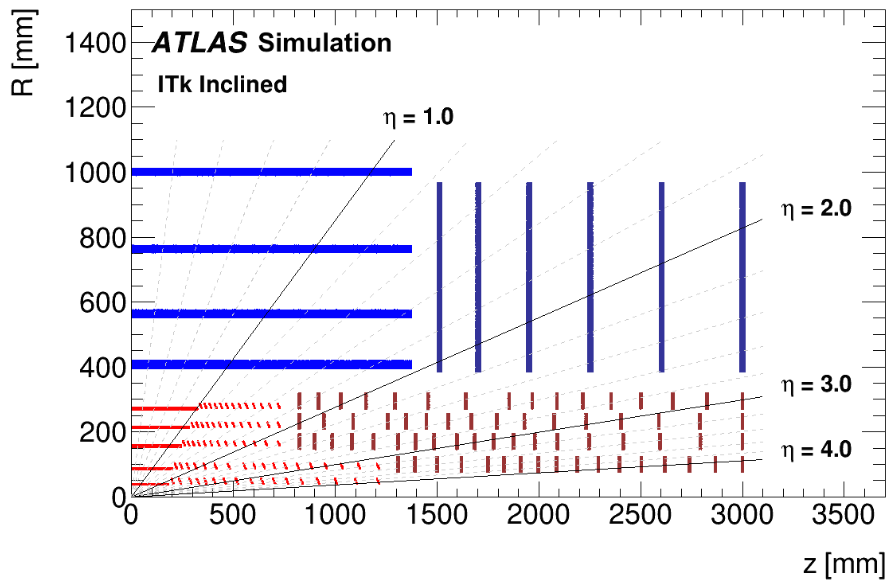
\includegraphics[width=.6\textwidth]{Pictures/ITklayout.png}
    \caption{ ITK layout as defined in ITk Technical Design Report \cite{ITktech}}
    \label{fig:ITklayout}
\end{figure}

\subsubsection{Building ITk Strip barrel staves}
At Brookhaven National Laboratory (BNL), I made key contributions to the ITk Strip barrel stave assembly effort. The goal of stave assembly is to glue silicon modules to carbon fiber stave cores within a 25 $\mu$m tolerance. Brookhaven is responsible for assembly of 200 ITk staves and their accurate assembly is necessary for the ITk to reduce uncertainty on track positions as well as to ensure a symmetric detector. I was tasked with co-creating a stave assembly software system through LABView to automatically calibrate required module positions, apply a layer of adhesive gel, and guide a user in accurately placing a module into its specified location. This project was highly collaborative and evolved further after I left the laboratory, but the overall process remains unchanged.

The basic design of the Inner Tracker for both barrel and endcap components is the same---a carbon fiber core (containing titanium cooling pipes) is covered on each side with co-cured kapton service tapes. The carbon fiber core is designed to reduce material inside the detector and the similar design in the barrel and endcap adds to simplicity. Silicon detector modules are glued to the stave cores. Similar silicon strip detectors have been used previously in both ATLAS and CMS, but have never covered so much fiducial area. The modules consist of one silicon sensor and one or two low-mass integrated circuit chips. Module design has optimized producibility and low cost while maintaining readout goals. Overall module design is the same in barrel and endcap regions, while strip lengths and geometries vary. Components of a short-strip barrel module are shown in Figure \ref{fig:module}. Each barrel stave core needs to be ``loaded" with 14 modules, as shown in the assembled electrical prototype in Figure \ref{fig:stave}.

\begin{figure}[!h]
        \centering
    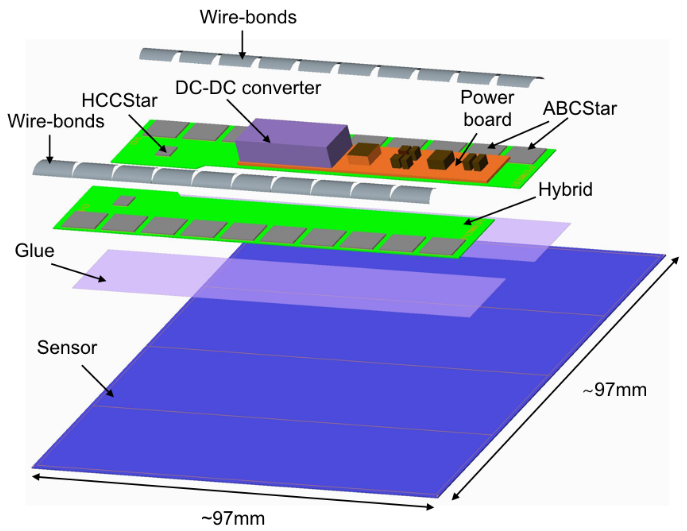
\includegraphics[width=.4\textwidth]{Pictures/ITkmodule.png}
    \caption{Short-strip barrel module components \cite{ITktech}}
    \label{fig:module}
\end{figure}
 
\begin{figure}[!h]
        \centering
    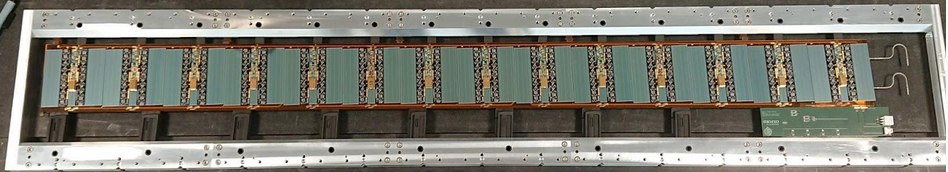
\includegraphics[width=.8\textwidth]{Pictures/electricalstave.png}
    \caption{Electrical stave prototype at Brookhaven National Laboratory (G. van Nieuwenhuizen)}
    \label{fig:stave}
\end{figure}

Brookhaven National Laboratory is one of two sites responsible for assembling barrel staves. Assembly procedures are tested with the production of numerous prototypes including a thermo-mechanical double-sided stave and a fully operational electrical stave. The thermo-mechanical prototype was later used for various thermal tests, including infrared imaging. The electrical stave was used for testing the full electrical read-out. Stave assembly is composed of three main parts: system calibration, module placement, and survey of results. 

Staves at BNL are assembled on a granite table housing an Aerotech XYZ Stage accurate to the micron level. The stage is equipped with a 10-megapixel camera that gives real-time feedback to a nearby computer and a glue dispenser. The stave assembly software system is implemented by a user who interacts with a LABView graphical user interface and monitors progress. The stave is fixed to optical rails drilled into the granite table. Calibrations are completed to accurately place modules in their correct positions. These include camera calibrations to test the optimal working point, focus, and pixel-to-micron conversion. Next, the position of the stave with relation to the XYZ stage is calibrated. Transforming coordinates of the XYZ stage to that of the stave requires locating a fixed point on the stave core as well as the angle of the stave relative to the XYZ stage. Pattern matching algorithms find the exact locations of particular features on the stave core and allow calculation of required positions for all modules based on specifications. Once specified, module positions are calculated, calibrations are completed and it is time to apply glue and attach modules. 

Next, an epoxy (SE4445) is loaded into the glue dispenser on the XYZ-stage which is connected to a vaccuum controlled by the LABView software system. The epoxy is automatically dispensed in lines to cover $\approx$ 60\% of area under the module. Then the module is lifted with a custom-made ``pick-up" tool which uses vacuum applied to module corners to hold the module in place and move it to the needed position along the optical rails. Using real-time feedback from the software system and its pattern matching algorithm, the user is directed on how to fine tune module position using knobs on the ``pick-up" tool. Markings etched in the silicon sensor at each corner are used to position the module accurately. The output of the module alignment GUI is shown in Figure \ref{fig:modulealignment}. When the module is within specifications it is lowered into position above the epoxy and held in place for 24 hours until the glue has completely dried.

\begin{figure}[!h]
        \centering
    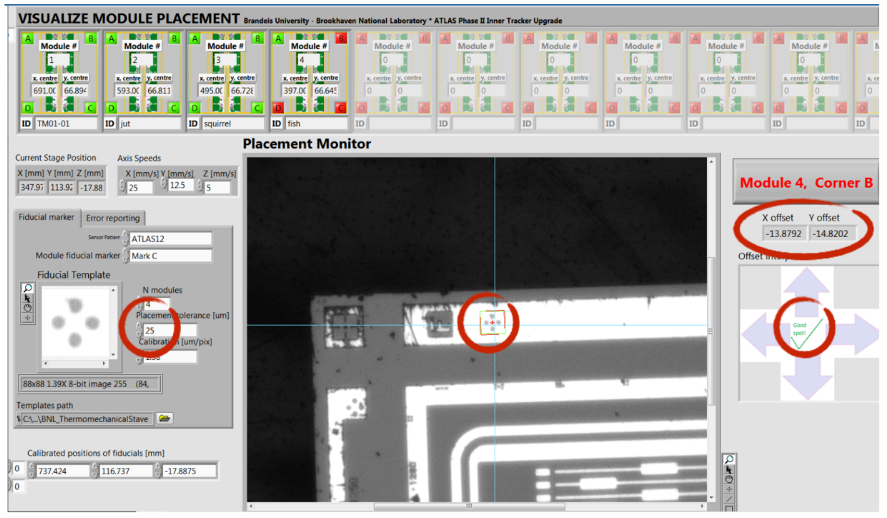
\includegraphics[width=.6\textwidth]{Pictures/labviewscreen.png}
    \caption{GUI interface showing etched marking on module corner located in real-time to guide user on how to adjust module position (H. Herde)}
    \label{fig:modulealignment}
\end{figure}

After the glue has set, a final survey of module positions is recorded using pattern matching to find positions of etched markings on each module corner. These results are saved into an ITk database and checked for any biases. After module placement on the stave is complete, the loaded stave is moved to another station in the lab for wirebonding so that all data from the modules can be read-out to stave-wide electronics. The module assembly system has been successful at placing modules accurately for all prototypes, achieving specification requirements for almost all modules. Results of the first prototype stave's module placement are shown in Figure \ref{fig:placementresults}. While a few module corners are slightly out of the ideal range, the majority are well within specifications. Throughout prototype assembly, issues and inefficiencies were found and corrected. New hardware, like an improved glue system and temperature monitoring, were also added. The methods described continue to be in use now and will be utilized for the production of 200 ITk staves at BNL starting in 2021. 

\begin{figure}[!h]
        \centering
    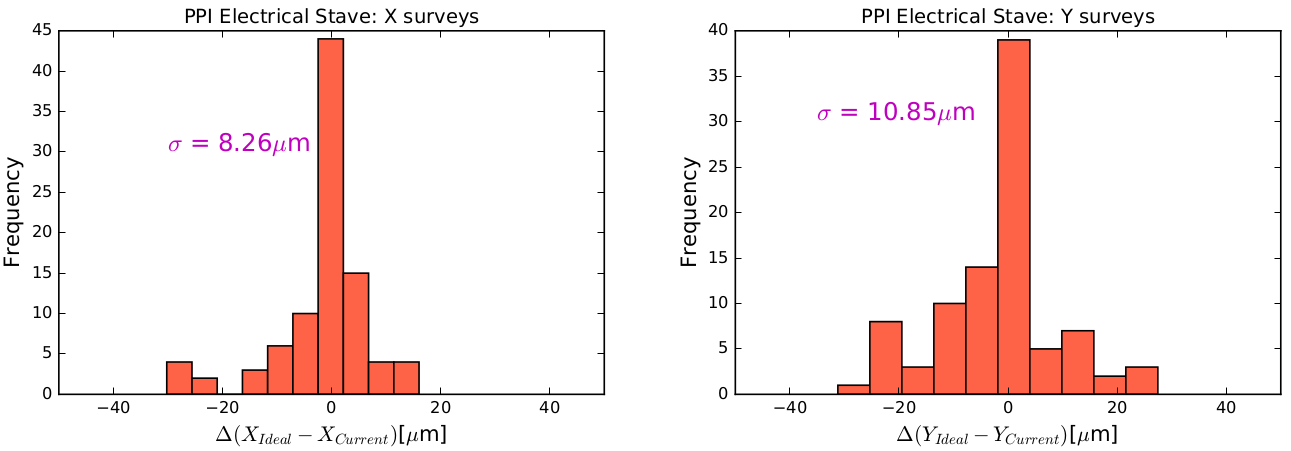
\includegraphics[width=.8\textwidth]{Pictures/placementresults.png}
    \caption{Histograms show difference between ideal and final position of each module corner. Left shows difference from specification in X and right in Y (P. Bhattarai)}
    \label{fig:placementresults}
\end{figure}

\subsubsection{IR Testing of ITk Strip barrel staves}
The first full US stave prototype was the thermo-mechanical stave built in the summer of 2017.  Building this stave was the first test of stave assembly procedures and the results proved that the module placement algorithm we developed worked. This stave was also used to test the thermal and mechanical properties of a fully loaded barrel stave. Multiple studies were conducted, including thermal measurements using thermistors and IR imaging, thermal cycling and thermal shock tests, mechanical studies, and bending tests. I will give a short summary of IR imaging tests, as these were another focus of my time at BNL. 

The thermo-mechanical (TM) stave consists of 13 modules mounted on each side. The modules used are thermo-mechanical, which means that instead of the usual readout chips their hybrids employed copper resistors to mimic the power dissipation and location of the chips. The powerboard can vary the TM hybrid power dissipation of each module individually. Three thermistors were mounted on each TM module, one on the DC-DC converter and one on each of the two hybrids. A custom End-of-Substructure (EoS) card is attached to a RaspberryPi and Arduino to power on or off each module.  
 
Thermal testing of barrel staves had a few main goals: to validate Finite Element Analysis (FEA) simulations by testing that all temperature trends are as we expect, to make sure that individual modules do not exhibit abnormal thermal behavior, and finally to check that loaded staves can cope with large changes in temperature they might face during operation. I will highlight a few key results which demonstrate that each of these goals have been accomplished. 

Thermal measurements were taken both through the mounted thermistors on each module and through IR imaging. IR imaging provides information about the entirety of the loaded stave, rather than at just a few module positions so provides a more complete picture. The loaded stave was spray-painted black with a high emissivity, low conductivity black paint since silicon is transparent to the IR camera spectrum (8--14 $\mu$m). In order to image the entire stave core, the IR camera was attached to rails above and pulled at a constant speed with an external motor as it recorded a video. The frames were then stitched together into one image. A section of the painted stave is shown in Figure \ref{fig:paintedstave}.  

\begin{figure}[!h]
        \centering
    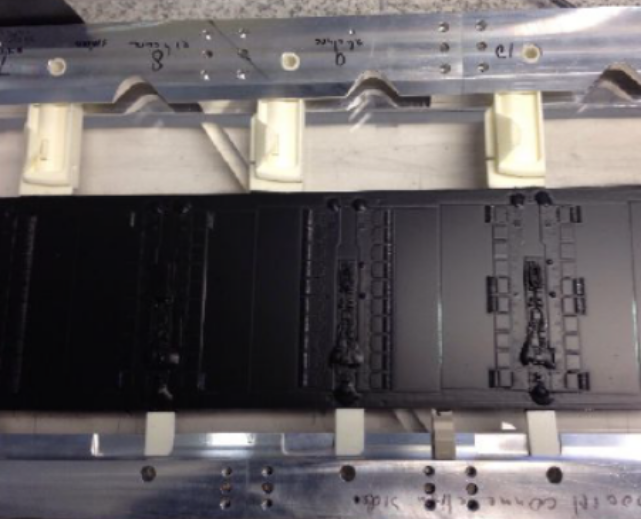
\includegraphics[width=.4\textwidth]{Pictures/paintedstave.png}
    \caption{Portion of the thermo-mechanical stave after being spray-painted for increased emissivity}
    \label{fig:paintedstave}
\end{figure}

FEA simulations for the thermal performance of a stave were completed by Prof. Graham Beck at Queen Mary University of London. These calculations quickly became intractable if convection was included so conditions of the stave and coolant were adjusted to minimize convective constributions or make sure that the total electrical power and power absorbed into the coolant were identical. At BNL, we adjusted the coolant temperature until we obtained the convective power minimization and then recorded module temperatures under these conditions. These results were compared to the FEA simulations by averaging hybrid temperatures recorded through IR imaging and recording thermistor readings. These comparisons are shown in Figure \ref{fig:FEAcompare}. The measurements show very good agreement with FEA calculations, within 5\% of the expected values.

\begin{figure}[!h]
        \centering
    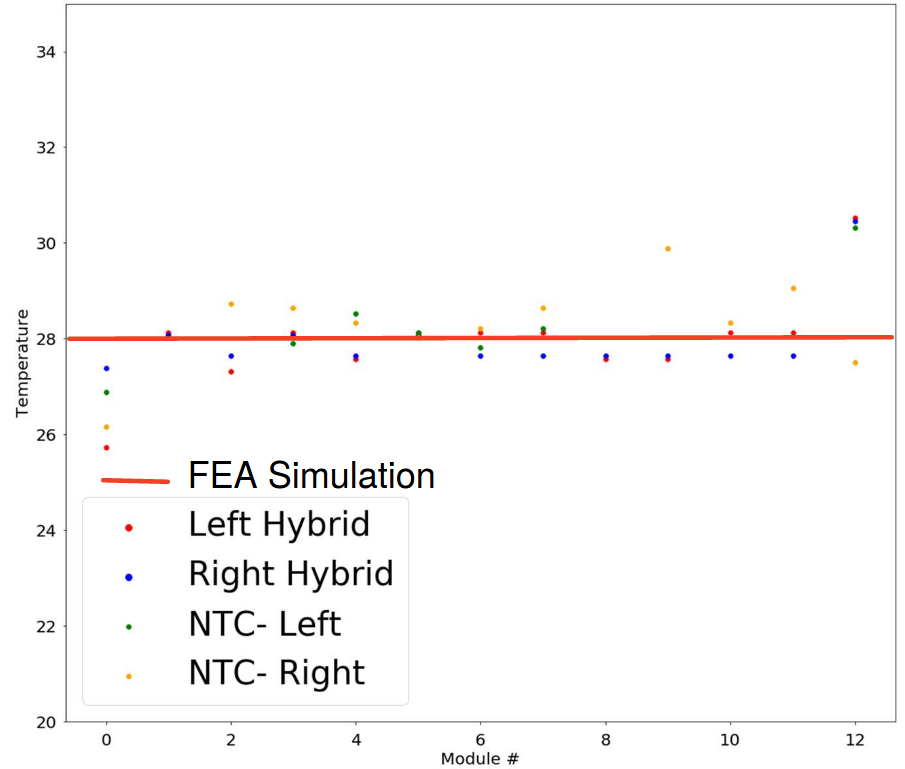
\includegraphics[width=.4\textwidth]{Pictures/FEAcompare.png}
    \caption{IR measurements, thermistor measurements, and FEA simulations for the TM stave are compared. Agreement with FEA simulation within 5\%.}
    \label{fig:FEAcompare}
\end{figure} 

During module assembly some slight variations were tested, including varying glue thickness below modules, glue curing time, and DC-DC converter types. Modules with and without these variations were compared at varying coolant temperatures and output power settings. Overall, no significant difference in module temperature change was observed for any of these assembly modifications. Stave thermal properties are thus robust to such assembly modifications. Figure \ref{fig:IRimagetotal} shows a full IR image of the fully loaded stave. It is clear that there are no obvious module-to-module variations in silicon, hybrid, or DC-DC converter temperature. The module sensors increase in temperature as they get closer to the EoS, which is expected since it dissipates power to the stave.

\begin{figure}[!h]
        \centering
    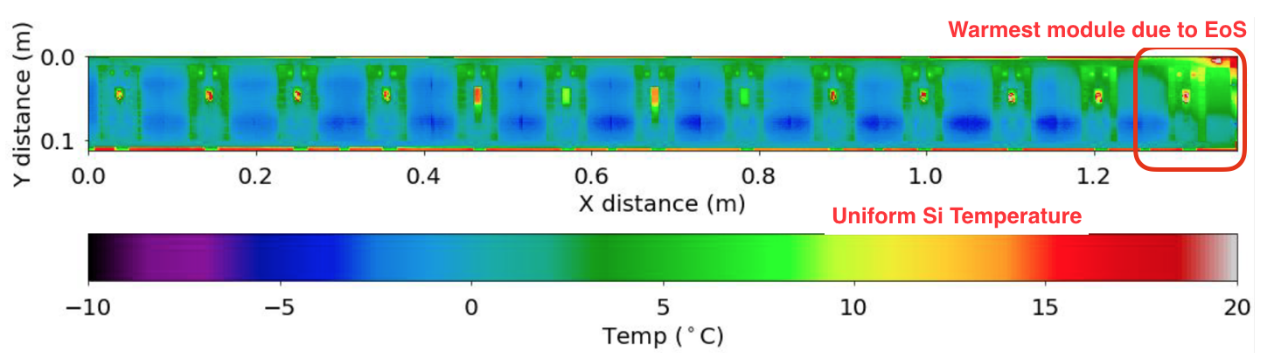
\includegraphics[width=.8\textwidth]{Pictures/IRimagetotal.png}
    \caption{IR image of fully loaded thermo-mechanical stave}
    \label{fig:IRimagetotal}
\end{figure} 
 
The thermo-mechanical stave was pushed to limits beyond what we would expect loaded staves to encounter during operation and never exhibited unexpected behavior. Thermal cycles, thermal shocks and bend tests showed the loaded stave to be robust against temperature variation and that the carbon fiber core is as stiff as it was prior to loading. Another test was how neighboring modules would perform if one module malfunctioned and was powered off. Figure \ref{fig:moduleoff} (top) shows the temperature of each module when one of them (fourth to the left) is turned off. The rest of the modules continue to operate normally and temperature changes from the unpowered module do not propagate very far. The bottom image in the figure shows the reverse of the stave when a module is powered off (fourth from the right). The temperature effects are greater on the module directly below than those adjacent to, which is expected due to material differences. 

\begin{figure}[!h]
        \centering
    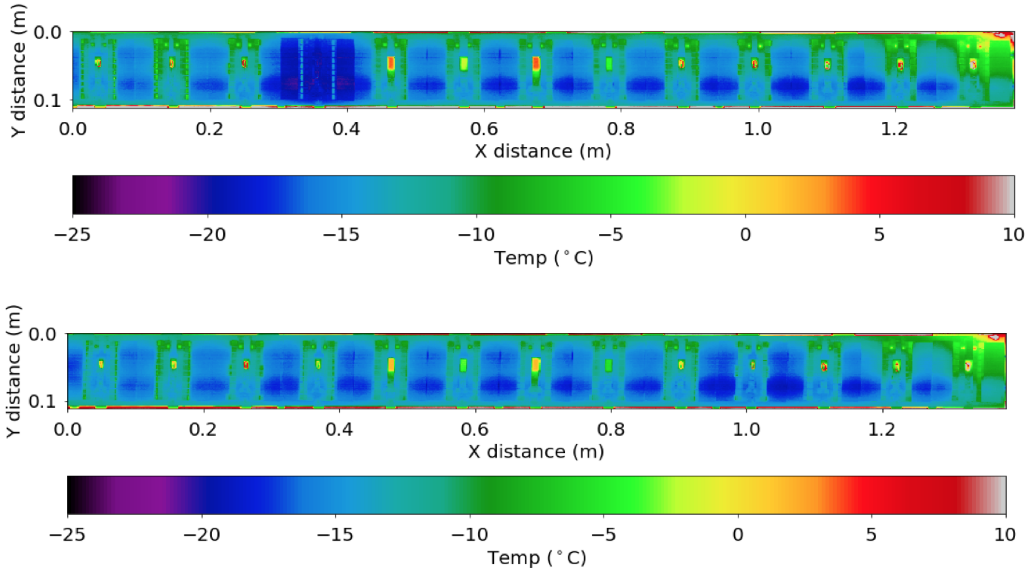
\includegraphics[width=.7\textwidth]{Pictures/moduleoff.png}
    \caption{IR image of fully loaded thermo-mechanical stave}
    \label{fig:moduleoff}
\end{figure}

My experiences on ATLAS detector upgrades for the HL-LHC provided context for the bulk of my thesis research. This project provided me with in depth and hands-on knowledge of the ATLAS detector and its component parts, as well as the scale of effort required to build new detector components. I have an abiding appreciation for the people and technology necessary for data-taking at the LHC, both of which make measurements like the Higgs cross-section detailed in this thesis possible.
